

\documentclass[11pt,compress,t,notes=noshow, xcolor=table]{beamer}
\usepackage[]{graphicx}\usepackage[]{color}
% maxwidth is the original width if it is less than linewidth
% otherwise use linewidth (to make sure the graphics do not exceed the margin)
\makeatletter
\def\maxwidth{ %
  \ifdim\Gin@nat@width>\linewidth
    \linewidth
  \else
    \Gin@nat@width
  \fi
}
\makeatother

\definecolor{fgcolor}{rgb}{0.345, 0.345, 0.345}
\newcommand{\hlnum}[1]{\textcolor[rgb]{0.686,0.059,0.569}{#1}}%
\newcommand{\hlstr}[1]{\textcolor[rgb]{0.192,0.494,0.8}{#1}}%
\newcommand{\hlcom}[1]{\textcolor[rgb]{0.678,0.584,0.686}{\textit{#1}}}%
\newcommand{\hlopt}[1]{\textcolor[rgb]{0,0,0}{#1}}%
\newcommand{\hlstd}[1]{\textcolor[rgb]{0.345,0.345,0.345}{#1}}%
\newcommand{\hlkwa}[1]{\textcolor[rgb]{0.161,0.373,0.58}{\textbf{#1}}}%
\newcommand{\hlkwb}[1]{\textcolor[rgb]{0.69,0.353,0.396}{#1}}%
\newcommand{\hlkwc}[1]{\textcolor[rgb]{0.333,0.667,0.333}{#1}}%
\newcommand{\hlkwd}[1]{\textcolor[rgb]{0.737,0.353,0.396}{\textbf{#1}}}%
\let\hlipl\hlkwb

\usepackage{framed}
\makeatletter
\newenvironment{kframe}{%
 \def\at@end@of@kframe{}%
 \ifinner\ifhmode%
  \def\at@end@of@kframe{\end{minipage}}%
  \begin{minipage}{\columnwidth}%
 \fi\fi%
 \def\FrameCommand##1{\hskip\@totalleftmargin \hskip-\fboxsep
 \colorbox{shadecolor}{##1}\hskip-\fboxsep
     % There is no \\@totalrightmargin, so:
     \hskip-\linewidth \hskip-\@totalleftmargin \hskip\columnwidth}%
 \MakeFramed {\advance\hsize-\width
   \@totalleftmargin\z@ \linewidth\hsize
   \@setminipage}}%
 {\par\unskip\endMakeFramed%
 \at@end@of@kframe}
\makeatother

\definecolor{shadecolor}{rgb}{.97, .97, .97}
\definecolor{messagecolor}{rgb}{0, 0, 0}
\definecolor{warningcolor}{rgb}{1, 0, 1}
\definecolor{errorcolor}{rgb}{1, 0, 0}
\newenvironment{knitrout}{}{} % an empty environment to be redefined in TeX

\usepackage{alltt}
\newcommand{\SweaveOpts}[1]{}  % do not interfere with LaTeX
\newcommand{\SweaveInput}[1]{} % because they are not real TeX commands
\newcommand{\Sexpr}[1]{}       % will only be parsed by R
\newcommand{\xmark}{\ding{55}}%


\usepackage[english]{babel}
\usepackage[utf8]{inputenc}

\usepackage{dsfont}
\usepackage{verbatim}
\usepackage{amsmath}
\usepackage{amsfonts}
\usepackage{amssymb}
\usepackage{bm}
\usepackage{csquotes}
\usepackage{multirow}
\usepackage{longtable}
\usepackage{booktabs}
\usepackage{enumerate}
\usepackage[absolute,overlay]{textpos}
\usepackage{psfrag}
\usepackage{algorithm}
\usepackage{algpseudocode}
\usepackage{eqnarray}
\usepackage{arydshln}
\usepackage{tabularx}
\usepackage{placeins}
\usepackage{tikz}
\usepackage{setspace}
\usepackage{colortbl}
\usepackage{mathtools}
\usepackage{wrapfig}
\usepackage{bm}
\usepackage{amsmath}
\usepackage{pifont}
\usepackage{xcolor} %colored math symbols

\usetikzlibrary{shapes,arrows,automata,positioning,calc,chains,trees, shadows}
\tikzset{
  %Define standard arrow tip
  >=stealth',
  %Define style for boxes
  punkt/.style={
    rectangle,
    rounded corners,
    draw=black, very thick,
    text width=6.5em,
    minimum height=2em,
    text centered},
  % Define arrow style
  pil/.style={
    ->,
    thick,
    shorten <=2pt,
    shorten >=2pt,}
}

\usepackage{subfig}

% Defines macros and environments
\usepackage{../../style/lmu-lecture}


\let\code=\texttt
\let\proglang=\textsf

\setkeys{Gin}{width=0.9\textwidth}

\setbeamertemplate{frametitle}{\expandafter\uppercase\expandafter\insertframetitle}

\usepackage{bbm}
% basic latex stuff
\newcommand{\pkg}[1]{{\fontseries{b}\selectfont #1}} %fontstyle for R packages
\newcommand{\lz}{\vspace{0.5cm}} %vertical space
\newcommand{\dlz}{\vspace{1cm}} %double vertical space
\newcommand{\oneliner}[1] % Oneliner for important statements
{\begin{block}{}\begin{center}\begin{Large}#1\end{Large}\end{center}\end{block}}


%new environments
\newenvironment{vbframe}  %frame with breaks and verbatim
{
 \begin{frame}[containsverbatim,allowframebreaks]
}
{
\end{frame}
}

\newenvironment{vframe}  %frame with verbatim without breaks (to avoid numbering one slided frames)
{
 \begin{frame}[containsverbatim]
}
{
\end{frame}
}

\newenvironment{blocki}[1]   % itemize block
{
 \begin{block}{#1}\begin{itemize}
}
{
\end{itemize}\end{block}
}

\newenvironment{fragileframe}[2]{  %fragile frame with framebreaks
\begin{frame}[allowframebreaks, fragile, environment = fragileframe]
\frametitle{#1}
#2}
{\end{frame}}


\newcommand{\myframe}[2]{  %short for frame with framebreaks
\begin{frame}[allowframebreaks]
\frametitle{#1}
#2
\end{frame}}

\newcommand{\remark}[1]{
  \textbf{Remark:} #1
}


\newenvironment{deleteframe}
{
\begingroup
\usebackgroundtemplate{
\includegraphics[width=\paperwidth,height=\paperheight]{../style/color/red.png}}
 \begin{frame}
}
{
\end{frame}
\endgroup
}
\newenvironment{simplifyframe}
{
\begingroup
\usebackgroundtemplate{
\includegraphics[width=\paperwidth,height=\paperheight]{../style/color/yellow.png}}
 \begin{frame}
}
{
\end{frame}
\endgroup
}\newenvironment{draftframe}
{
\begingroup
\usebackgroundtemplate{
\includegraphics[width=\paperwidth,height=\paperheight]{../style/color/green.jpg}}
 \begin{frame}
}
{
\end{frame}
\endgroup
}
% https://tex.stackexchange.com/a/261480: textcolor that works in mathmode
\makeatletter
\renewcommand*{\@textcolor}[3]{%
  \protect\leavevmode
  \begingroup
    \color#1{#2}#3%
  \endgroup
}
\makeatother


\input{../../latex-math/basic-math}
\input{../../latex-math/basic-ml}
\input{../../latex-math/ml-nn}

\newcommand{\titlefigure}{figure/gru_vs_lstm.png}
%modify picture
\newcommand{\learninggoals}{
  \item LSTM cell
  \item GRU cell
}

\title{Deep Learning}
\date{}



\begin{document}

\lecturechapter{Modern Recurrent Neural Networks}
\lecture{I2DL}



%%%%%%%%%%%%%%%%%%%%%%%%%%%%%%%%%%%%%%%%%%%%%%%%%%%%%%%%%%%%%%%%%%
%\begin{vbframe}{Long Short-Term Memory  (LSTM)}
%  \begin{itemize}
%    \item The LSTM provides a different way of dealing with vanishing gradients and modelling long-term dependencies.
%    \item A cell state $s^{[t]}$ is introduced, which can be manipulated by different \textbf{gates} to forget old information, add new information and read information out of it.
%    \item Each gate is a vector of the same size as the cell state and each element of the vector is a
%number between $0$ and $1$, with $0$ meaning \enquote{let nothing pass} and 1 \enquote{let everything pass}.
%    \item The gates are computed as a parametrized function of the previous hidden state $z^{[t-1]}$ and the input at the current time step $x^{[t]}$ multiplied by \textbf{gate-specific weights} and typically squashed through a sigmoid function into the range of $[0, 1]$.
%    \item The cell state allows the recurrent neural network to keep information over long time ranges. %and therefore overcome the vanishing gradient problem.
%  \end{itemize}
%\end{vbframe}
%%%%%%%%%%%%%%%%%%%%%%%%%%%%%%%%%%%%%%%%%%%%%%%%%%%%%%%%%%%%%%%%%%
%%%%%%%%%%%%%%%%%%%%%%%%%%%%%%%%%%%%%%%%%%%%%%%%%%%%%%%%%%%%%%%%%%

\section{Long Short-Term Memory (LSTM)}

\frame{
\frametitle{Long Short-Term Memory (LSTM)}
The LSTM provides a way of dealing with vanishing gradients and modelling long-term dependencies.
  \begin{figure}
    \only<1>{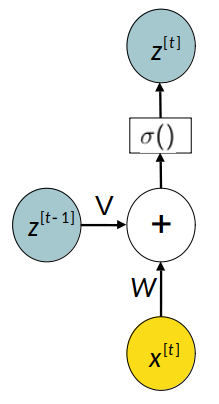
\includegraphics[width=2cm]{figure/vanilla_rnn.png}}%
    \only<2>{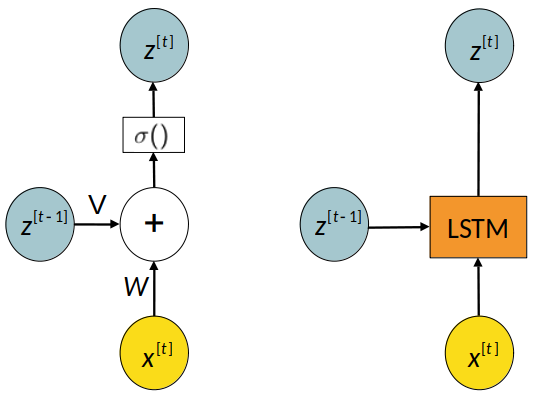
\includegraphics[width=5cm]{figure/vanilla_rnn_lstm.png}}%
\tiny{\\\only<2>{Left:} A simple RNN mechanism; \only<2>{Right: An LSTM cell}}
  \end{figure}
  \begin{itemize}
    \only<1-2>{\item Until now, we simply computed $$\mathbf{z}^{[t]} = \sigma(\mathbf{b} + \mathbf{V}^\top \mathbf{z}^{[t-1]} + \mathbf{W}^\top \xv^{[t]})$$}
    \only<2>{\item Now we introduce the LSTM cell, a small network on its own. }
  \end{itemize}
}
%%%%%%%%%%%%%%%%%%%%%%%%%%%%%%%%%%%%%%%%%%%%%%%%%%%%%%%%%%%%%%%%%%
%%%%%%%%%%%%%%%%%%%%%%%%%%%%%%%%%%%%%%%%%%%%%%%%%%%%%%%%%%%%%%%%%%
% \frame{
% \frametitle{Long Short-Term Memory - LSTM}
%   \begin{itemize}
%     \item[]
%   \end{itemize}
%   \begin{minipage}{0.51\textwidth}
%     \only<1-2>{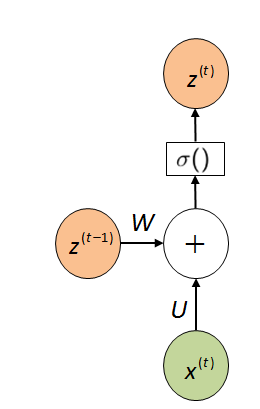
\includegraphics[width=2.5cm]{plots/vanilla_rnn.png}}%
%     \begin{itemize}
%       \only<1-2>{\item Untill now, we simply computed $$z^{[t]} = \sigma(b + Wz^{[t-1]} + Ux^{[t]})$$}
%       \only<2>{\item Now we introduce the lstm cell (this is where the fun begins).}
%     \end{itemize}
%   \end{minipage}\hfill
%   \vspace{-0.7cm}
%   \begin{minipage}{0.41\textwidth}
%     \only<1>{
\includegraphics[width=2.5cm]{plots/vanilla_lstm1.png}}%
%     \only<2>{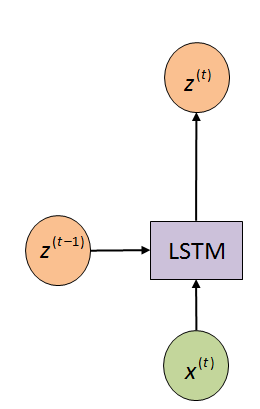
\includegraphics[width=2.5cm]{plots/vanilla_lstm2.png}}%
%     \begin{itemize}
%       \only<1-2>{\item[] \textcolor{white}{with} $$\textcolor{white}{z^{(t)} = \sigma(b + Wz^{[t-1]} + Ux^{[t]})}$$}
%       \only<2>{\item[] \textcolor{white}{Now we introduce the lstm cell (this is where the fun begins).}}
%     \end{itemize}
%   \end{minipage}
% }
%%%%%%%%%%%%%%%%%%%%%%%%%%%%%%%%%%%%%%%%%%%%%%%%%%%%%%%%%%%%%%%%%%
%%%%%%%%%%%%%%%%%%%%%%%%%%%%%%%%%%%%%%%%%%%%%%%%%%%%%%%%%%%%%%%%%%
\frame{

\frametitle{Long Short-Term Memory (LSTM)}

  \center
  \only<1>{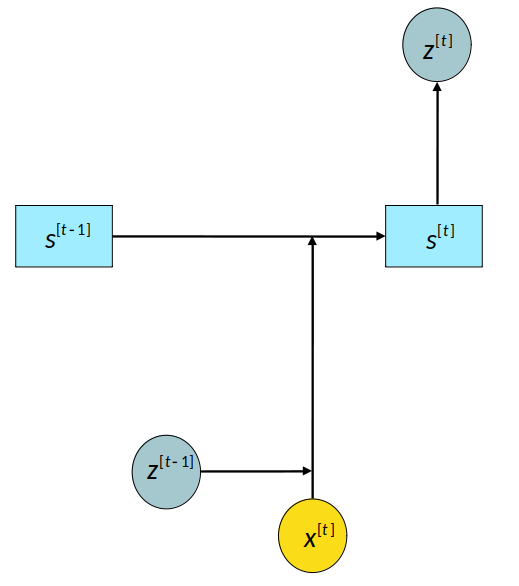
\includegraphics[width=3.5cm]{figure/lstm_1.png}}%
  \only<2>{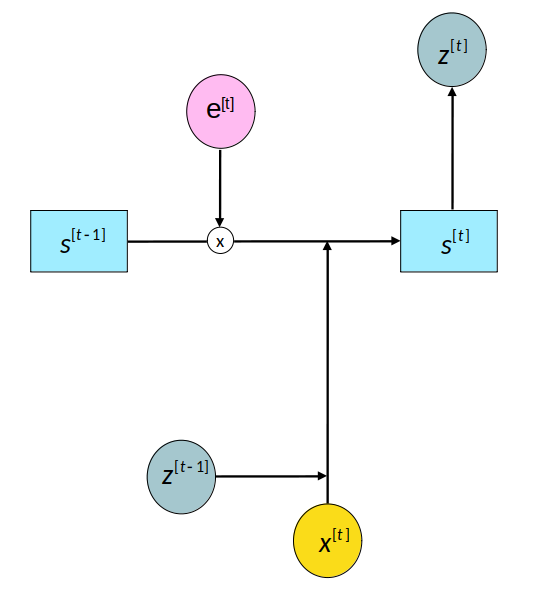
\includegraphics[width=3.5cm]{figure/lstm_2.png}}%
  \only<3-4>{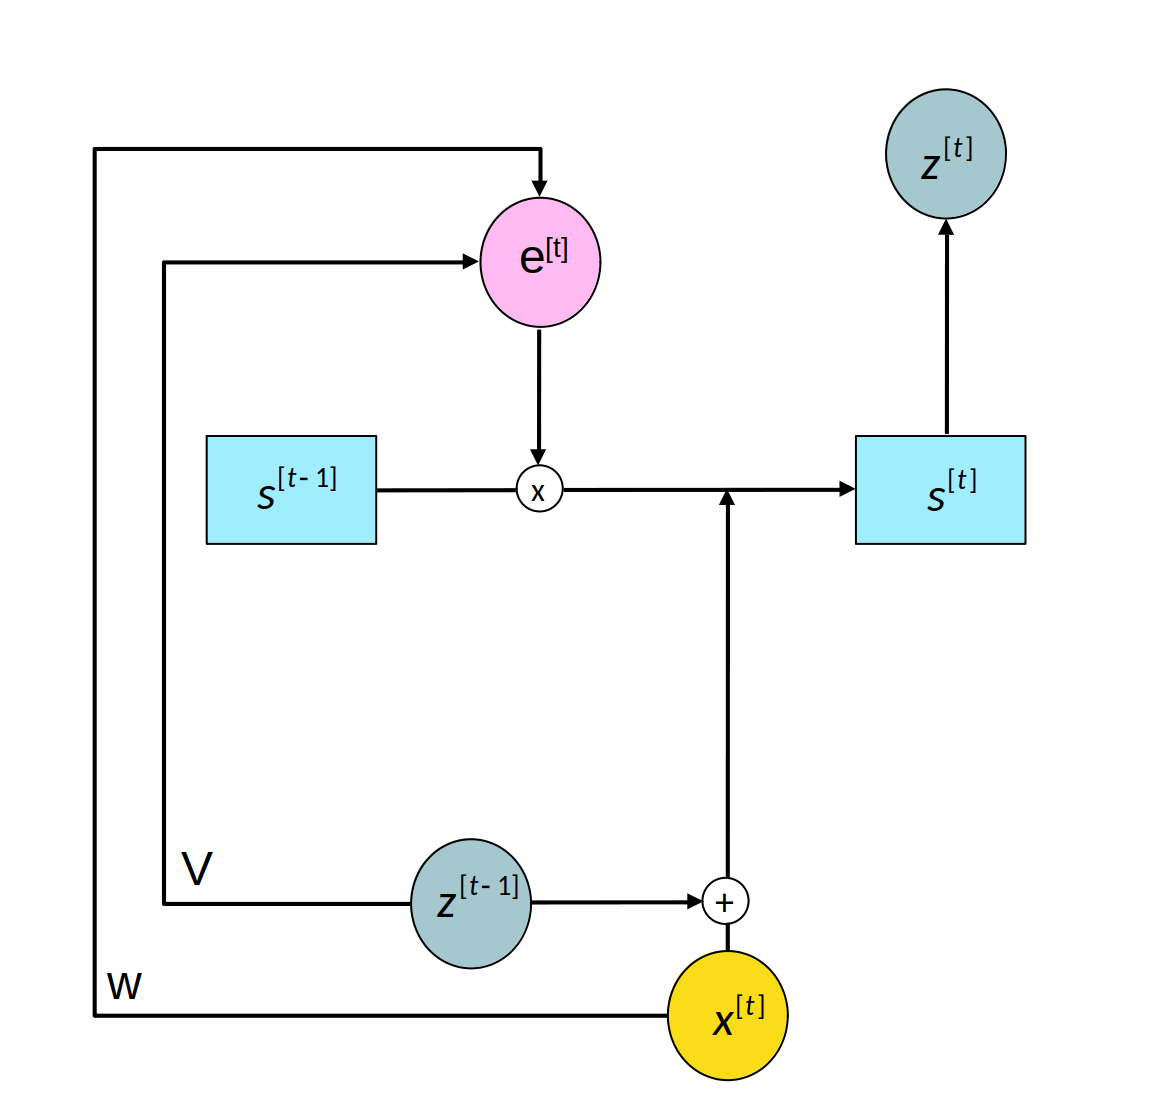
\includegraphics[width=4.75cm]{figure/lstm_3.png}}%
  \only<5-7>{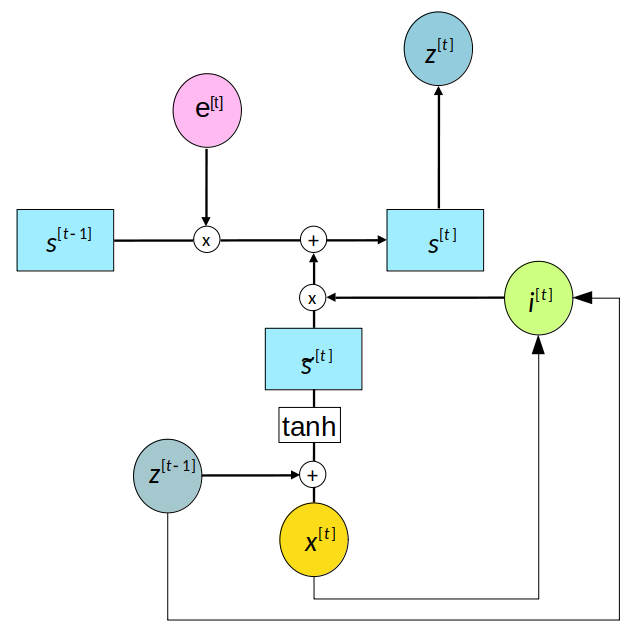
\includegraphics[width=4.75cm]{figure/lstm_4.png}}%
  \only<8-9>{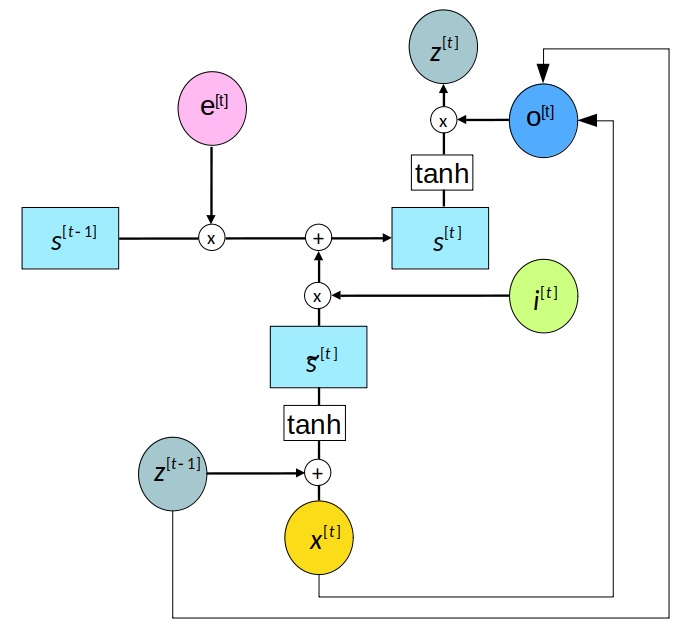
\includegraphics[width=4.75cm]{figure/lstm_5.png}}%
  
  \begin{itemize}

    \only<1>{\item The key to LSTMs is the \textbf{cell state} $\mathbf{s}^{[t]}$.}
    \only<1>{%\item The LSTM does have the ability to remove or add information to the cell state, carefully regulated by structures called gates.
    \item $\mathbf{s}^{[t]}$ can be manipulated by different \textbf{gates} to forget old information, add new information, and read information out of it.}
\only<1>{\item Each gate is a vector of the same size as $\mathbf{s}^{[t]}$ with elements between 0 ("let nothing pass") and 1 ("let everything pass").
}
    
    \only<2>{\item \textbf{Forget gate}  $\mathbf{e}^{[t]}$: indicates which information of the old cell state we should forget. 
    \item Intuition: Think of a model trying to predict the next word based on all the previous ones. The cell state might include the gender of the present subject, so that the correct pronouns can be used. When we now see a new subject, we want to forget the gender of the old one.}
    \only<3>{\item We obtain the forget gate by computing 
%    $$f^{[t]} = \sigma(b^{(f)} + V^{(f)T} z^{[t-1]} + W^{(f)T} x^{[t]})$$
    $$\mathbf{e}^{[t]} = \sigma(\mathbf{b}_{e} + \mathbf{V}_e^\top \mathbf{z}^{[t-1]} + \mathbf{W}_e^\top \xv^{[t]})$$}
    \only<3>{\item $\sigma()$ is  a sigmoid and $\mathbf{V}_e, \mathbf{W}_e$ are forget gate specific weights.}
    \only<4>{\item To compute the cell state $\mathbf{s}^{[t]}$, the first step is to multiply (element-wise) the previous cell state $\mathbf{s}^{[t-1]}$ by the forget gate $\mathbf{e}^{[t]}$. $$\mathbf{e}^{[t]} \odot \mathbf{s}^{[t-1]}, \text{ with } \mathbf{e}^{[t]} \in [0,1]$$}
    \only<5>{\item \textbf{Input gate} $\mathbf{i}^{[t]}$: indicates which new information should be added to  $\mathbf{s}^{[t]}$.}
    %\only<5>{\item We again incorporate the information in the previous hidden state $z^{[t-1]}$.}
    \only<5>{\item Intuition: In our example, this is where we add the new information about the gender of the new subject.}
   % \only<6>{\item The cell recurrent connection needs a function whose derivatives sustain for a long span to address the vanishing gradient problem.}
    \only<6>{\item The new information is given by $\tilde{\mathbf{s}}^{[t]} = \text{tanh}(\mathbf{b} + \mathbf{V}^\top \mathbf{z}^{[t-1]} + \mathbf{W}^\top \xv^{[t]}) \in [-1, 1]$.}
    \only<6>{\item The input gate is given by $\mathbf{i}^{[t]} = \sigma(\mathbf{b}_i + \mathbf{V}_i^\top \mathbf{z}^{[t-1]} + \mathbf{W}_i^\top \xv^{[t]}) \in [0,1]$.}
   \only<6>{\item $\mathbf{W}$ and $\mathbf{V}$ are weights of the new information, $\mathbf{W}_i$ and $\mathbf{V}_i$ the weights of the input gate.}
    \only<7>{\item Now we can finally compute the cell state $\mathbf{s}^{[t]}$: 
    $$\mathbf{s}^{[t]} = \mathbf{e}^{[t]} \odot \mathbf{s}^{[t-1]} + \mathbf{i}^{[t]} \odot \tilde{\mathbf{s}}^{[t]}$$}
    %\only<7>{\item[] By the way: this does not mean that our lstm is complete! }
   % \only<8>{\item In order to complete the lstm cell, one final ingredient is missing.}
   % \only<8>{\item The output of the LSTM cell will be a filtered version of our cell state.}
    \only<8>{\item %First, we run a sigmoid layer which decides what parts of the cell
   \textbf{Output gate} $\mathbf{o}^{[t]}$:  Indicates which information form the cell state is filtered.
   \item It is given by $\mathbf{o}^{[t]} = \sigma(\mathbf{b}_o + \mathbf{V}_o^\top \mathbf{z}^{[t-1]} + \mathbf{W}_o^\top \xv^{[t]})$, with specific weights $\mathbf{W}_o, \mathbf{V}_o$.}
    %\only<8>{\item }
    \only<9>{\item Finally, the new state $\mathbf{z}^{[t]}$ of the LSTM is a function of the cell state, multiplied by the output gate: $$\mathbf{z}^{[t]} = \mathbf{o}^{[t]} \odot \text{tanh}(\mathbf{s}^{[t]})$$}

  \end{itemize}

}





%%%%%%%%%%%%%%%%%%%%%%%%%%%%%%%%%%%%%%%%%%%%%%%%%%%%%%%%%%%%%%%%%%
\section{Gated Recurrent Units (GRU)}
\frame{
\frametitle{Gated Recurrent Units (GRU)}

   \begin{itemize}
     \item The key distinction between regular RNNs and GRUs is that the latter support gating of the hidden state. 
     \item Here, we have dedicated mechanisms for when a hidden state should be updated and also when it should be reset.
     \item These mechanisms are learned to: 
     \begin{itemize}
           \item avoid the vanishing/exploding gradient problem which comes with a standard recurrent neural network.
           \item solve the vanishing gradient problem by using an update gate and a reset gate. 
           \item control the information that flows into (update gate) and out of (reset gate) memory.
     \end{itemize}
   \end{itemize}
   
}
%%%%%%%%%%%%%%%%%%%%%%%%%%%%%%%%%%%%%%%%%%%%%%%%%%%%%%%%%%%%%%%%%%
\begin{vbframe}{Gated Recurrent Units (GRU)}
    \begin{figure}
      \centering
      \scalebox{0.38}{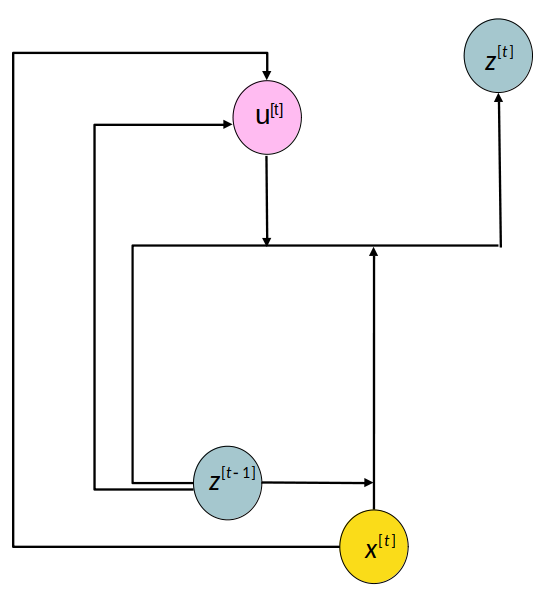
\includegraphics{figure/gru_1.png}}
      \caption{\footnotesize{Update gate in a GRU.}}
  \end{figure}
  \begin{itemize}
    %\item as shown by Figure1, given the current time step input $X_t$ and the hidden state of the previous time step $H_{t-1}$. The output is given by a fully connected layer with a sigmoid as its activation function.
    \item For a given time step $t$, the hidden state of the last time step is $\mathbf{z}^{[t-1]}$. The update gate $\mathbf{u}^{[t]}$ is computed as follows:
   \item $\mathbf{u}^{[t]} = \sigma(\mathbf{W}_{u}^\top \mathbf{x}^{[t]} + \mathbf{V}_{u}^\top \mathbf{z}^{[t-1]}  + \mathbf{b}_u)$
    \item We use a sigmoid to transform input values to $(0,1)$.
  \end{itemize}
\end{vbframe}

\begin{vbframe}{Gated Recurrent Units (GRU)}
    \begin{figure}
      \centering
      \scalebox{0.4}{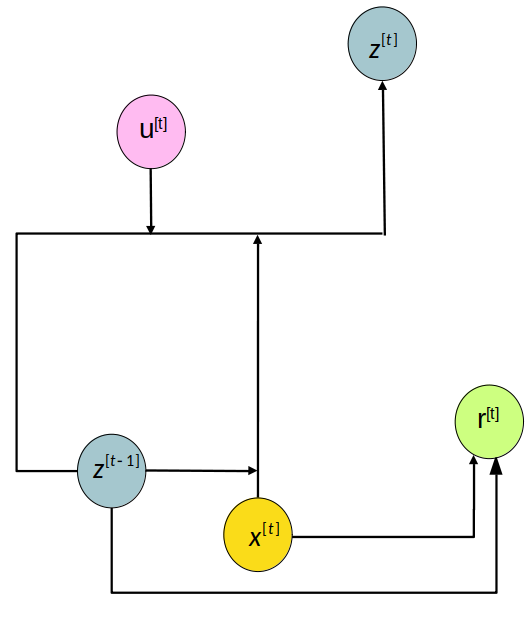
\includegraphics{figure/gru_2.png}}
      \caption{\footnotesize{Reset gate in a GRU.}}
  \end{figure}
  \begin{itemize}
    %\item as shown by Figure1, given the current time step input $X_t$ and the hidden state of the previous time step $H_{t-1}$. The output is given by a fully connected layer with a sigmoid as its activation function.
    \item Similarly, the reset gate $\mathbf{r}^{[t]}$ is computed as follows:
   \item $\mathbf{r}^{[t]} = \sigma(\mathbf{W}_{r}^\top \mathbf{x}^{[t]} +\mathbf{V}_{r}^\top \mathbf{z}^{[t-1]} + \mathbf{b}_r)$

  \end{itemize}
\end{vbframe}

%%%%%%%%%%%%%%%%%%%%%%%%%%%%%%%%%%%%%%%%%%%%%%%%%%%%%%%%%%%%%%%%%%
\begin{vbframe}{Gated Recurrent Units (GRU)}
     \begin{figure}
      \centering
      \scalebox{0.4}{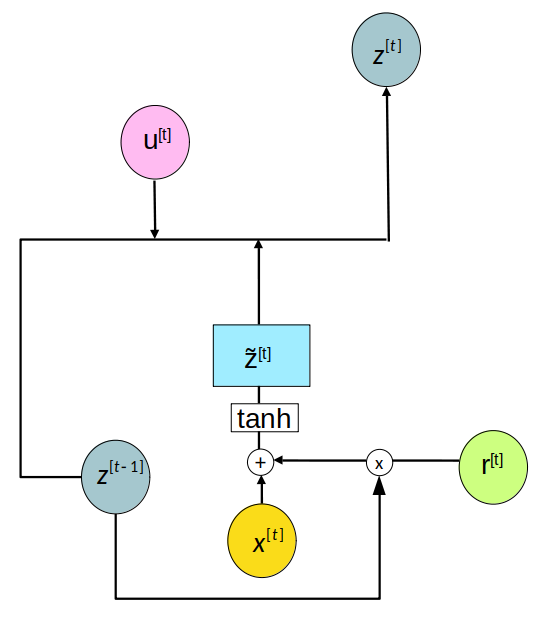
\includegraphics{figure/gru_25.png}}
      \caption{\footnotesize{Hidden state computation in GRU. Multiplication is carried out elementwise.}}
  \end{figure}
  \begin{itemize}
   %\item If we want to be able to reduce the influence of the previous states we can multiply $H_{t−1}$ with $R_t$ elementwise. 
  % Whenever the entries in the reset gate $R_t$ are close to 1, we recover a conventional RNN. For all entries of the reset gate $R_t$ that are close to 0, the hidden state is the result of an MLP with $X_t$ as input. Any pre-existing hidden state is thus reset to defaults. This leads to the following candidate hidden state (it is a candidate since we still need to incorporate the action of the update gate).

  \item  $\tilde{\mathbf{z}}^{[t]} = \tanh(\mathbf{W}_{z}^\top \mathbf{x}^{[t]} + \mathbf{V}_{z}^\top \left(\mathbf{r}^{[t]} \odot \mathbf{z}^{[t-1]}\right)  + \mathbf{b}_z).$
   \item In a conventional RNN, we would have an hidden state update of the form:  $\mathbf{z}^{[t]} = \tanh(\mathbf{W}_{z}^\top \mathbf{x}^{[t]} + \mathbf{V}_{z}^\top \mathbf{z}^{[t-1]} + \mathbf{b}_z).$
   \end{itemize}
  
\end{vbframe}
%%%%%%%%%%%%%%%%%%%%%%%%%%%%%%%%%%%%%%%%%%%%%%%%%%%%%%%%%%%%%%%%%%
\begin{vbframe}{Gated Recurrent Units (GRU)}
 \begin{figure}
      \centering
      \scalebox{0.4}{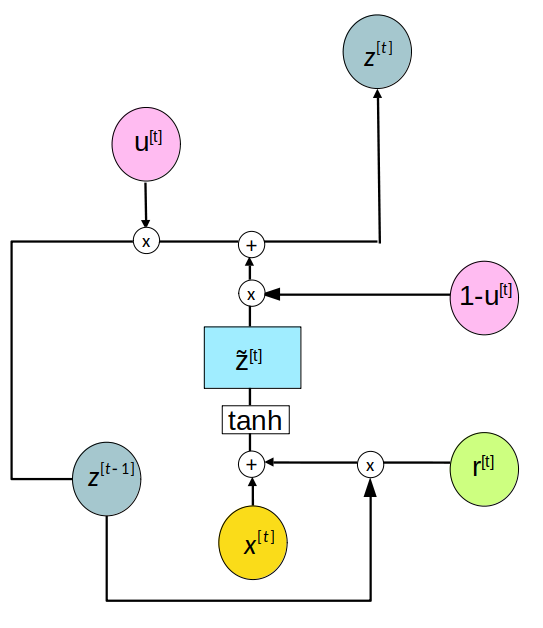
\includegraphics{figure/gru_3.png}}
      \caption{\footnotesize{Update gate in a GRU. The multiplication is carried out elementwise.}}
  \end{figure}
  
  \begin{itemize}
  \item The update gate $\mathbf{u}^{[t]}$ determines how much the old state $\mathbf{z}^{[t-1]}$ and the new candidate state $\tilde{\mathbf{z}}^{[t]}$ is used. 
  \item $\mathbf{z}^{[t]} = \mathbf{u}^{[t]} \odot \mathbf{z}^{[t-1]}  + (1 - \mathbf{u}^{[t]}) \odot \tilde{\mathbf{z}}^{[t]}.$
  \end{itemize}
  \begin{figure}
      \centering
      \scalebox{0.3}{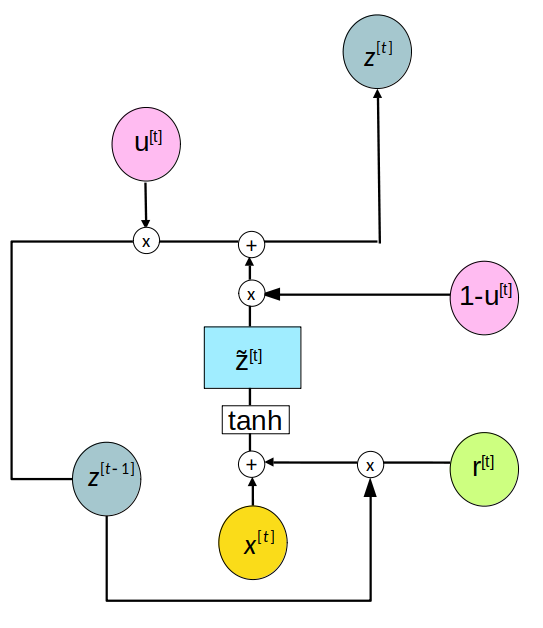
\includegraphics{figure/gru_3.png}}
      \caption{\footnotesize{GRU}}
  \end{figure}
 
  These designs can help us to eleminate the vanishing gradient problem in RNNs and capture better dependencies for time series with large time step distances. In summary, GRUs have the following two distinguishing features:
  \begin{itemize}
    \item Reset gates help capture short-term dependencies in time series.
    \item Update gates help capture long-term dependencies in time series.
  \end{itemize}
\end{vbframe}

\begin{vbframe}{GRU vs LSTM}
  \begin{figure}
     \centering
      \scalebox{0.8}{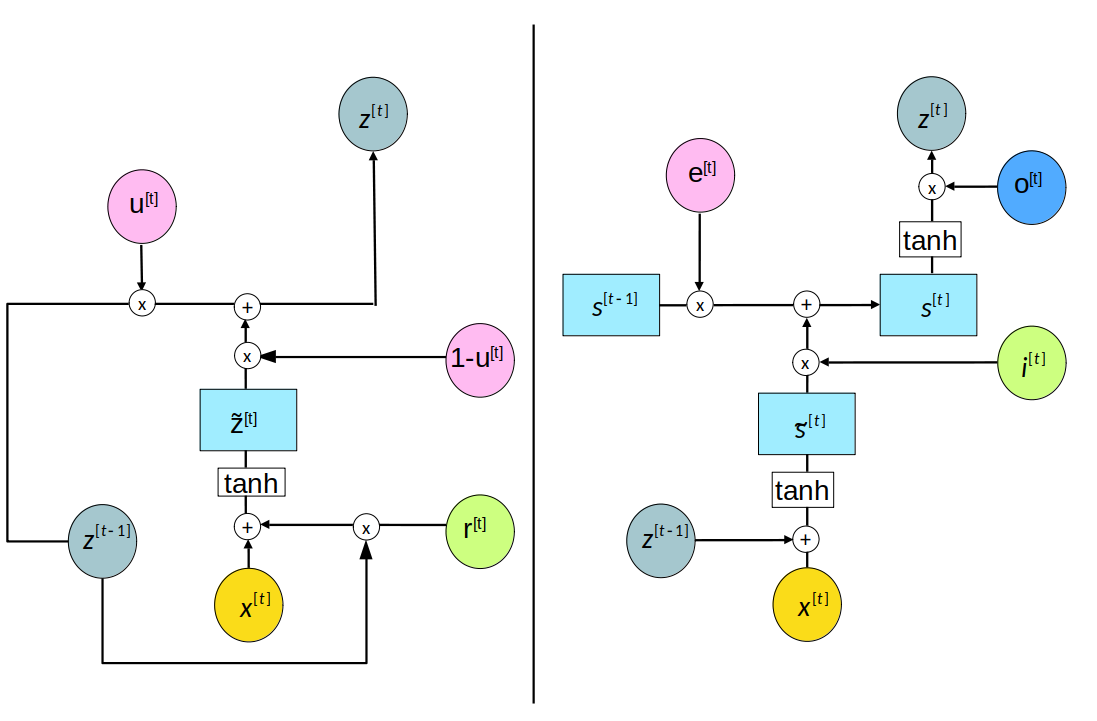
\includegraphics{figure/gru_vs_lstm.png}}
      \caption{\footnotesize{GRU vs LSTM}}
  \end{figure}

\end{vbframe}

%%%%%%%%%%%%%%%%%%%%%%%%%%%%%%%%%%%%%%%%%%%%%%%%%%%%%%%%%%%%%%%%%%



%%%%%%%%%%%%%%%%%%%%%%%%%%%%%%%%%%%%%%%%%%%%%%%%%%%%%%%%%%%%%%%%%%
%%%%%%%%%%%%%%%%%%%%%%%%%%%%%%%%%%%%%%%%%%%%%%%%%%%%%%%%%%%%%%%%%%
%%%%%%%%%%%%%%%%%%%%%%%%%%%%%%%%%%%%%%%%%%%%%%%%%%%%%%%%%%%%%%%%%%
% \begin{vbframe}{RNN with output recurrence}
%   \begin{figure}
%     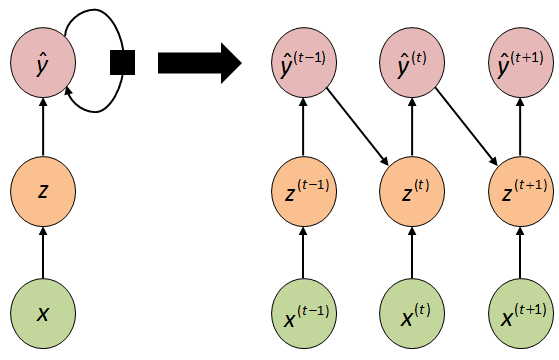
\includegraphics[width=5.5cm]{plots/output_recurrence.png}
%   \end{figure}
%   \begin{itemize}
%     \item Such an RNN is less powerful (can express a smaller set of functions).
%     \item However, it may be easier to train because each time step it can be trained in isolation from the others, allowing greater parallelization during training.
%   \end{itemize}
% \end{vbframe}
% %%%%%%%%%%%%%%%%%%%%%%%%%%%%%%%%%%%%%%%%%%%%%%%%%%%%%%%%%%%%%%%%%%
% %%%%%%%%%%%%%%%%%%%%%%%%%%%%%%%%%%%%%%%%%%%%%%%%%%%%%%%%%%%%%%%%%%
% \begin{vbframe}{Teacher Forcing}
%   \begin{itemize}
%     \item Teacher forcing is a procedure that emerges from the maximum likelihood criterion, in which during training the model receives the ground truth output $y^{[t]}$ as input at time $[t + 1]$.
%   \end{itemize}
%   \begin{minipage}{0.51\textwidth}
%     \begin{figure}
%       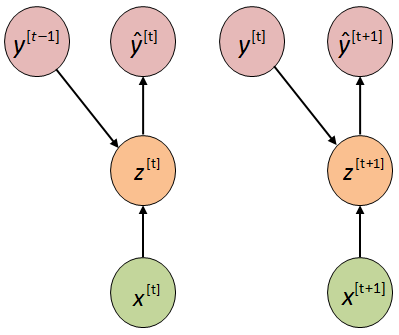
\includegraphics[width=3.8cm]{plots/teacher_forcing_train.png}
%     \end{figure}  
%     \begin{itemize}
%       \item At training time
%     \end{itemize}
%   \end{minipage}
%   \begin{minipage}{0.45\textwidth}
%     \begin{figure}
%       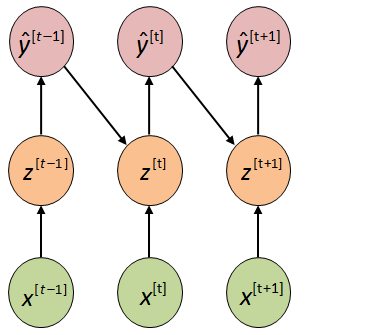
\includegraphics[width=3.8cm]{plots/teacher_forcing_test.png}
%     \end{figure} 
%     \begin{itemize}
%       \item At testing time
%     \end{itemize}
%   \end{minipage}
% \end{vbframe}
%%%%%%%%%%%%%%%%%%%%%%%%%%%%%%%%%%%%%%%%%%%%%%%%%%%%%%%%%%%%%%%%%%
%%%%%%%%%%%%%%%%%%%%%%%%%%%%%%%%%%%%%%%%%%%%%%%%%%%%%%%%%%%%%%%%%%
% \begin{vbframe}{One-output RNN}
%   \begin{itemize}
%     \item Recurrent Neural Networks do not need to have an output at each time step, instead they can
% only have outputs at a few time steps.
%     \item A common variant is an RNN with only one output at the end of the sequence.
%     \item Information from the whole input sequence is incorporated into the final hidden state, which is then used to create an output, e.g. a sentiment (\enquote{positive}, \enquote{neutral} or \enquote{negative}) for a movie review.
%     \item  Other applications of such an architecture are sequence labeling, e.g. classify an article into different categories (\enquote{sports}, \enquote{politics} etc.)
%   \end{itemize}
% \framebreak
%   \begin{figure}
%     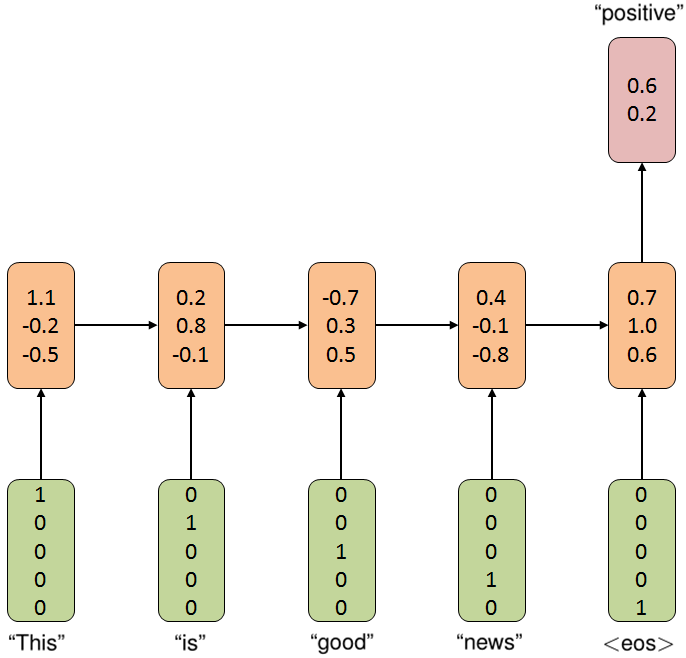
\includegraphics[width=6.5cm]{plots/one_output_rnn.png}
%     \caption{A Recurrent Neural Network with one output at the end of the sequence. Such a
% model can be used for sentiment analysis ($<$eos$>$ = \enquote{end of sequence}).}
%   \end{figure}
% \end{vbframe}
%%%%%%%%%%%%%%%%%%%%%%%%%%%%%%%%%%%%%%%%%%%%%%%%%%%%%%%%%%%%%%%%%%
% \begin{frame} {Stacked RNNs}
% \end{frame}

%%%%%%%%%%%%%%%%%%%%%%%%%%%%%%%%%%%%%%%%%%%%%%%%%%%%%%%%%%%%%%%%%%
%%%%%%%%%%%%%%%%%%%%%%%%%%%%%%%%%%%%%%%%%%%%%%%%%%%%%%%%%%%%%%%%%%
% \begin{vbframe}{Recursive neural networks}
%   \begin{itemize}
%     \item Recursive Neural Networks are a generalization of Recurrent Neural Networks. 
%     \item A tree structure instead of a chain structure is used for the computations of the RNN.
%     \item A fixed set of weights is repeatedly applied to the nodes of the tree.
%     \item Recursive neural networks have been successfully applied to sentiment analysis!
%   \end{itemize}
% \framebreak  
%   \begin{figure}
%     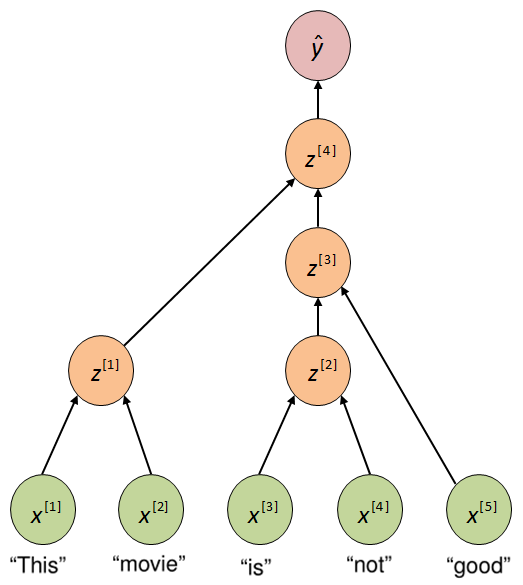
\includegraphics[width=5.8cm]{plots/recursive_neural_network.png}
%     \caption{A recursive neural network}
%   \end{figure} 
% \end{vbframe}
%%%%%%%%%%%%%%%%%%%%%%%%%%%%%%%%%%%%%%%%%%%%%%%%%%%%%%%%%%%%%%%%%
%%%%%%%%%%%%%%%%%%%%%%%%%%%%%%%%%%%%%%%%%%%%%%%%%%%%%%%%%%%%%%%%%%
%%%%%%%%%%%%%%%%%%          REFERENCES          %%%%%%%%%%%%%%%%%%
%%%%%%%%%%%%%%%%%%%%%%%%%%%%%%%%%%%%%%%%%%%%%%%%%%%%%%%%%%%%%%%%%%
% \begin{vbframe}
% \frametitle{References}
% \footnotesize{
% \begin{thebibliography}{99}
% %%%%%%%%%%%%%%%%%%%%%%%%%%%%%%%%%%
% \bibitem[Ian Goodfellow et al., 2016]{1} Ian Goodfellow, Yoshua Bengio and Aaron Courville (2016)
% \newblock Deep Learning
% \newblock \emph{\url{http://www.deeplearningbook.org/}}
% %%%%%%%%%%%%%%%%%%%%%%%%%%%%%%%%%
% %\bibitem[Michael Nguyen, 2018]{1} Michael Nguyen (2018)
% %\newblock Illustrated Guide to LSTM's and GRU's: A step by step explanation
% %newblock \emph{\url{https://towardsdatascience.com/illustrated-guide-to-lstms-and-gru-s-a-step-by-step-explanation-44e9eb85bf21}}
% %%%%%%%%%%%%%%%%%%%%%%%%%%%%%%%%%
% \end{thebibliography}
% }
% \end{vbframe}
%%%%%%%%%%%%%%%%%%%%%%%%%%%%%%%%%%%%%%%%%%%%%%%%%%%%%%%%%%%%%%%%%%
%%%%%%%%%%%%%%%%%%%%%%%%%%%%%%%%%%%%%%%%%%%%%%%%%%%%%%%%%%%%%%%%%%

\endlecture
\end{document}
